\section{Structs}



\subsection{Binary Search Tree - BST}

\subsubsection{Concept}

A \textbf{Binary Search Tree (BST)} is a data structure used in computer science to organize and store data in an ordered manner. Conceptually, a tree must adhere to specific criteria to be considered a binary search tree:

Each node in a Binary Search Tree has, at most, two children: a left child and a right child. The left child contains values smaller than the parent node, while the right child contains values larger than the parent node.

This hierarchical structure allows for efficient search, insertion, and deletion operations on the data stored in the tree. In time complexity analysis, the efficiency of a BST is linear in relation to the height of the tree. Furthermore, the best time for basic operations—insertion, deletion, and search—takes $O(\log n)$ for $n$ nodes. In the worst case, when the tree degenerates (becoming similar to a linked list), the time can reach $O(n)$.

\subsubsection{Implementation}

\begin{itemize}
    \item \underline{\textbf{Insert Function:}}

    For inserting a word into the tree, the main idea is to preserve the existing structure. Thus, the insertion process is divided into two primary cases: the word already exists in the tree, or it is a new word. This distinction is made using the previously implemented `Search` function.

    In the first case, where the word already belongs to a node in the tree, the function searches for the ID of the text to be inserted within the `documentIds` list of the corresponding node. If the ID is already present, no action is taken. Otherwise, the ID for that text is added to the list. As an optimization, the list of IDs is traversed in reverse. Since texts are inserted in ascending order, this means that if the word was already present in the text, its ID would have been the last one added, thus saving computational time. However, to ensure the code remains functional regardless of the file insertion order, the decision was made to retain a full loop through the list.

    On the other hand, if the word is not already in the tree, it must be added as a child node of a leaf. Since the `Search` function already stores the parent node, one simply compares the new word with the parent node's word to determine if the new node will be inserted as a left or right child. A special case occurs when the tree is empty (i.e., the parent is null); in this scenario, the new node is set as the root of the tree.
    
\end{itemize}

\subsection{AVL}

\subsubsection{Concept}

An \textbf{AVL Tree} is a \textbf{Binary Search Tree (BST)} that distinguishes itself by being self-balancing. The key characteristic of an AVL tree is that for any node in the tree, the absolute difference between the heights of its left and right subtrees must be at most 1. This difference is known as the \textit{balancing factor}.

Whenever an operation (such as insertion or deletion) causes an imbalance---that is, the balancing factor of a node becomes greater than 1---the tree performs a rebalancing. This process is carried out through specific rotations, which reorganize the nodes to restore the balancing property.

This self-balancing mechanism ensures that operations like insertion, search, and deletion are executed with a time complexity of $O(\log n)$, where $n$ is the number of nodes in the tree. This is crucial for maintaining efficiency, even in trees with a large volume of data. Furthermore, it prevents the degeneration that can occur in a standard BST.


\subsubsection{Implementation}

\begin{itemize}
  \item \underline {\textbf{Function BalancingFactor:}}
  
  In short, the function calculates the balancing factor of a given node by finding the difference between the heights of the right and left subtrees.
  
  \item \underline {\textbf{Function Rotates:}}
  
  As part of the tree's rebalancing, it is necessary to perform rotations on parts of it. Thus, these functions execute rotations in each direction. The transformations performed by each function will be visually represented in the following graphs:

  \begin{itemize}
    \item \textit{\textbf{First Case:}} The node is the root and has no parent.    \begin{center}
    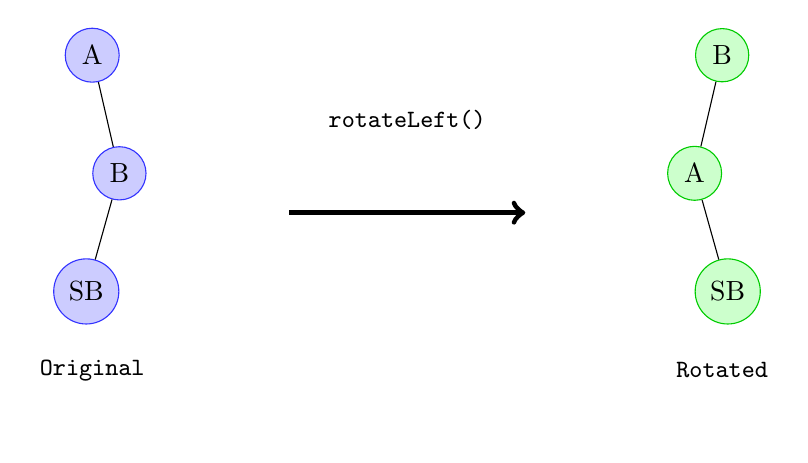
\begin{tikzpicture}[
          level distance=15mm, sibling distance=15mm,
          every node/.style={circle, draw, minimum size=8mm, font=\ttfamily\small}
    ]
    
    \begin{scope}[xshift=-4cm, every node/.style={circle, draw=blue!80, fill=blue!20}]
        \node {A}
            child[right] {node {B}
                child [left]{node {SB}} 
            }
        ;
    \end{scope}
    
    \begin{scope}[xshift=4cm, every node/.style={circle, draw=green!80!black, fill=green!20}]
    \node {B}
      child [left]{node {A}
        child[right] {node {SB}}
      };
    \end{scope}
    
    \draw[->, very thick, line width=2pt] (-1.5,-2.0) -- (1.5,-2.0) 
        node[midway, above, yshift=0.2pt, draw=none, fill=none] {rotateLeft()};
        
    \node[draw=none, fill=none] at (-4, -4) {\textbf{Original} };
    \node[draw=none, fill=none] at (4, -4) {\textbf{Rotated} };
    
    \end{tikzpicture}
    \end{center}

    \item \textit{\textbf{Second Case:}} The node is a left child.  \begin{center}
    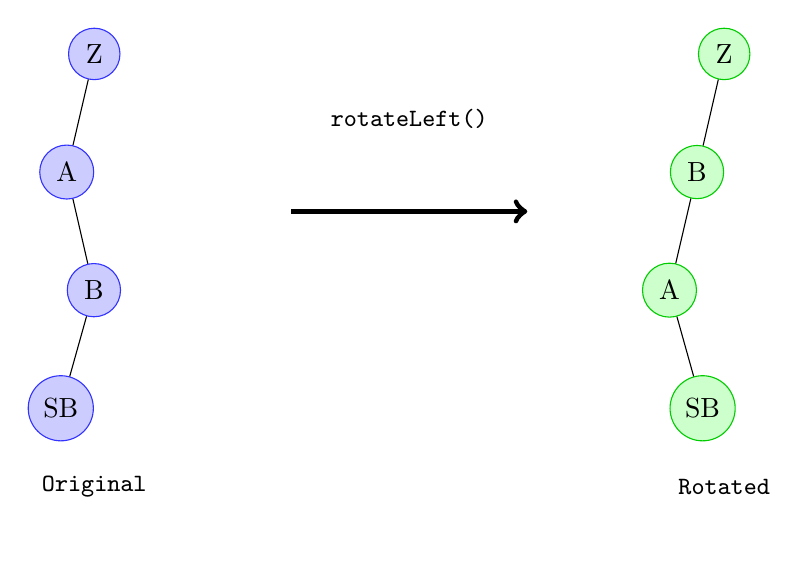
\begin{tikzpicture}[
          level distance=15mm, sibling distance=15mm,
          every node/.style={circle, draw, minimum size=8mm, font=\ttfamily\small}
    ] 
      \begin{scope}[xshift=-4cm, every node/.style={circle, draw=blue!80, fill=blue!20}]
        \node {Z}
          child [left] {
            node {A}
              child [right] {
                node {B}
                  child [left]{node {SB}}
              }
          };

        \end{scope}
        
        \begin{scope}[xshift=4cm, every node/.style={circle, draw=green!80!black, fill=green!20}]
        \node {Z}
          child [left] {
            node {B}
              child [left] {
                node {A}
                  child[right] {node {SB}}
              }
          };

        \end{scope}
        
        \draw[->, very thick, line width=2pt] (-1.5,-2.0) -- (1.5,-2.0) 
            node[midway, above, yshift=0.2pt, draw=none, fill=none] {rotateLeft()};
        
                \node[draw=none, fill=none] at (-4, -5.5) {\textbf{Original} };
        \node[draw=none, fill=none] at (4, -5.5) {\textbf{Rotated} };
        
      \end{tikzpicture}
    \end{center}

      \item \textit{\textbf{Third Case:}} The node is a right child.        
          \begin{center}
    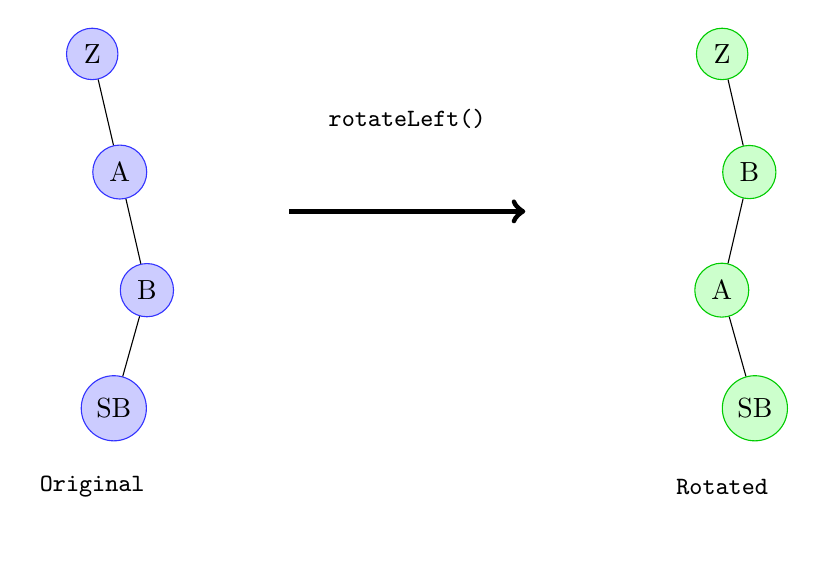
\begin{tikzpicture}[
          level distance=15mm, sibling distance=15mm,
          every node/.style={circle, draw, minimum size=8mm, font=\ttfamily\small}
    ] 
      \begin{scope}[xshift=-4cm, every node/.style={circle, draw=blue!80, fill=blue!20}]
        \node {Z}
          child [right] {
            node {A}
              child [right] {
                node {B}
                  child [left]{node {SB}}
              }
          };

        \end{scope}
        
        \begin{scope}[xshift=4cm, every node/.style={circle, draw=green!80!black, fill=green!20}]
        \node {Z}
          child [right] {
            node {B}
              child [left] {
                node {A}
                  child[right] {node {SB}}
              } 
          };

        \end{scope}
        
        \draw[->, very thick, line width=2pt] (-1.5,-2.0) -- (1.5,-2.0) 
            node[midway, above, yshift=0.2pt, draw=none, fill=none] {rotateLeft()};
        
                \node[draw=none, fill=none] at (-4, -5.5) {\textbf{Original} };
        \node[draw=none, fill=none] at (4, -5.5) {\textbf{Rotated} };
        
      \end{tikzpicture}
    \end{center}

    The rotations presented are derived from the left rotation operation, where the node to be rotated is $A$ and $SB$ represents a subtree. For a right rotation, a similar but mirrored logic is applied. It is important to note that the cases shown do not occur in valid binary search trees, but they constitute the base cases for the rotation algorithms.

    Furthermore, there are what are known as double rotations, which are used when an imbalance occurs at two levels---for example, when a node is a right child, but its own child is a left child (or vice-versa). In these situations, the \texttt{rotateRightLeft} and \texttt{rotateLeftRight} functions are used to restore the tree's balance.

    \item \textit{\textbf{Rotate Left Right:}} Double Rotation
    \begin{center}
    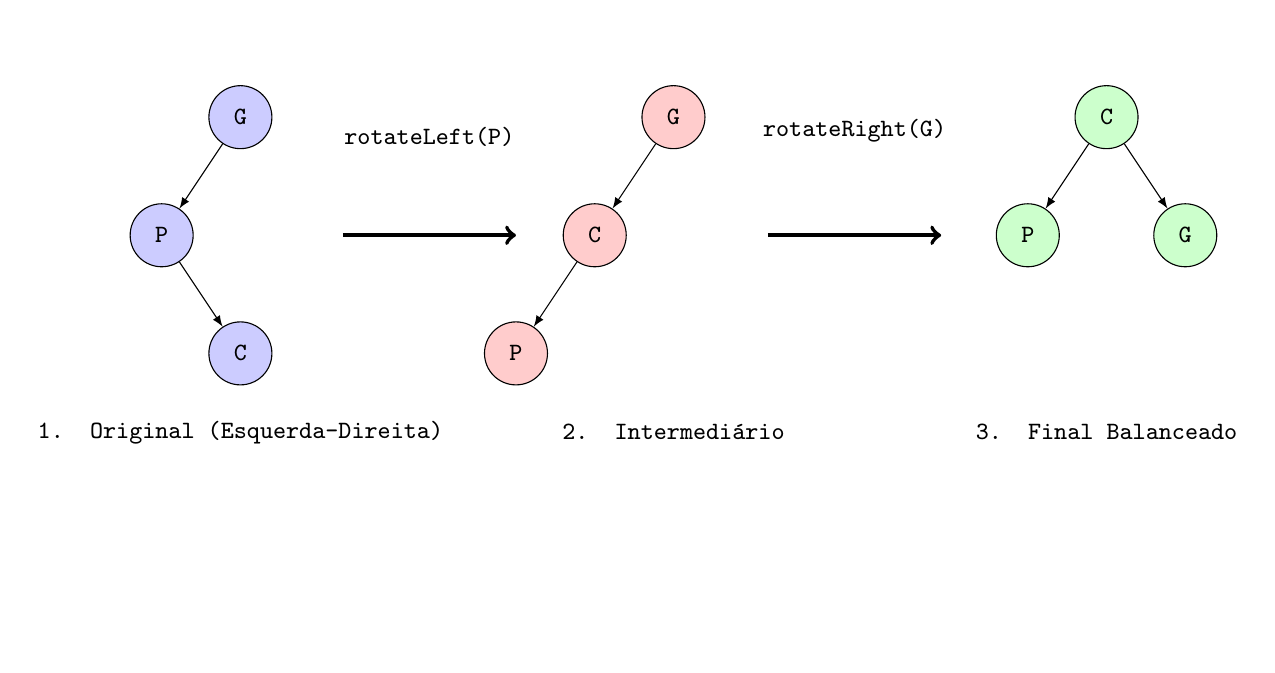
\begin{tikzpicture}[
      level distance=15mm, sibling distance=20mm,
      every node/.style={circle, draw, minimum size=8mm, font=\ttfamily\small},
      edge from parent/.style={draw, -latex}
    ]
    
    \begin{scope}[xshift=-5.5cm]
        \node (G) [fill=blue!20] {G}
            child {node (P) [fill=blue!20] {P}
                child[missing]
                child {node (C) [fill=blue!20] {C}}
            }
            child[missing];
        \node[draw=none, fill=none] at (0, -4) {\textbf{1. Original (Esquerda-Direita)}};
    \end{scope}
    
    \draw[->, very thick, line width=1.5pt] (-4.2cm,-1.5cm) -- (-2cm,-1.5cm) 
        node[midway, above, draw=none, fill=none] {rotateLeft(P)};
    
    \begin{scope}[xshift=0cm]
        \node (G) [fill=red!20] {G}
            child {node (C) [fill=red!20] {C}
                child {node (P) [fill=red!20] {P}}
                child[missing]
            }
            child[missing];
        \node[draw=none, fill=none] at (0, -4) {\textbf{2. Intermediário}};
    \end{scope}
    
    \draw[->, very thick, line width=1.5pt] (1.2cm,-1.5cm) -- (3.4cm,-1.5cm) 
        node[midway, above, draw=none, fill=none] {rotateRight(G)};
    
    \begin{scope}[xshift=5.5cm]
        \node (C) [fill=green!20] {C}
            child {node (P) [fill=green!20] {P}}
            child {node (G) [fill=green!20] {G}};
        \node[draw=none, fill=none] at (0, -4) {\textbf{3. Final Balanceado}};
    \end{scope}
    
    \end{tikzpicture}
    \end{center}
    
  \end{itemize}

  \item \underline{\textbf{Balance Function:}}

  The \texttt{balance} function is responsible for checking if a given node violates the balancing property of an AVL tree. To do this, it first calculates the node's balancing factor. If the absolute value of this factor is greater than 1, it indicates an imbalance and, therefore, the need for a rotation.

  Next, the function determines if the imbalance is in the left or right subtree and checks whether a single or double rotation is needed based on the balancing factor of the corresponding child. After applying the appropriate rotation, the function returns the new, balanced node.

  \item \underline{\textbf{Insert Function:}}

  In general, insertion into an AVL tree follows the same logic as insertion into a BST, divided into two cases: the word is already in the tree, or it is a new entry. After this check, the balancing process begins.

  If the word does not yet exist in the tree, after its insertion as a child of a leaf node, a recursive check is performed from the new node's parent up to the root. At each step, it verifies if the current node maintains the AVL balancing property. If the tree remains balanced, no action is necessary; otherwise, the \texttt{balance} function is called to restore the local balance.

  This process ensures that, by the end of the insertion, all nodes above the new element---all the way to the root---are also balanced. In this way, the entire tree structure continues to adhere to the AVL balancing rules, maintaining its efficiency for search, insertion, and deletion operations.

\end{itemize}














\subsection{Red-Black Tree - RBT}

\subsubsection{Concept}

A \textbf{Red-Black Tree} is a variation of the binary search tree that uses a set of properties to stay balanced. This guarantees that insertion, search, and deletion operations have logarithmic time complexity, even in the worst cases.

To ensure this balance, each node in the tree is assigned a color---either \textcolor{red}{red} or \textbf{black}---and after each modification (insertion or deletion), the tree's balance is restored through rotations and recolorings as needed.

A Red-Black Tree must obey the following properties:
\begin{enumerate}
    \item \underline{Node Color:} Every node is either red or black.
    \item \underline{Root Property:} The root of the tree is always black.
    \item \underline{Red Property:} A red node cannot have red children (i.e., there are no two consecutive red nodes on any path).
    \item \underline{Black Property:} Every path from a given node to any of its descendant NIL nodes contains the same number of black nodes.
    \item \underline{Leaf Property:} All leaves (NIL nodes) are black.
\end{enumerate}

\subsubsection{Implementation}

\begin{itemize}
    \item \underline{\textbf{Transplant Function:}}

    The \texttt{transplant} auxiliary function is responsible for replacing one node, $u$, with another node, $v$, in the tree. In other words, it makes the parent of $u$ point to $v$. Furthermore, if $v$ is not null, the function updates the parent pointer of $v$ to point to the former parent of $u$.

    \item \underline{\textbf{FixInsert Function:}}
    
    Given the properties of a Red-Black Tree, we first need to determine the color of the newly added node, which we will call $z$. As established, $z$ can only be black or red. Let's see what happens in each case:
    
    If $z$ is black: 
    \begin{itemize}
        \item It violates Property 4, unless $z$ is the root.
    \end{itemize}
    
    If $z$ is red:
    \begin{itemize}
        \item Property 4 is maintained.
        \item If its parent is red, Property 3 is violated.
        \item If it is the root, Property 2 is violated.
    \end{itemize}
    
    Therefore, by convention, every node initially inserted into a Red-Black Tree is colored red. When this insertion leads to a violation of the tree's properties, the issue can be resolved by handling a series of specific cases.
    
    In addressing these violations, three main cases (and their symmetric counterparts) are distinguished.
    \begin{itemize}
    \item \textit{\textbf{First Case:} The uncle of the newly inserted node $z$ is red.}

    Since $z$ is inserted as a red node, its parent, $p$, might also be red. This configuration violates the Red Property of a Red-Black Tree (a red node cannot have a red child). Assuming that the uncle of $z$, denoted by $y$, is also red, we perform a recoloring to fix the violation.

    In this situation, we assume that the grandparent of $z$, denoted by $g$, was black before the insertion---which guarantees the tree was valid up to that point. The fix consists of recoloring both $p$ and $y$ to black, and $g$ to red. This resolves the local conflict.

    However, this recoloring might have introduced a new conflict at the level of the grandparent, $g$, if its parent is also red. Therefore, the verification and correction must be applied recursively up the tree until all properties are restored.

        \begin{center}
        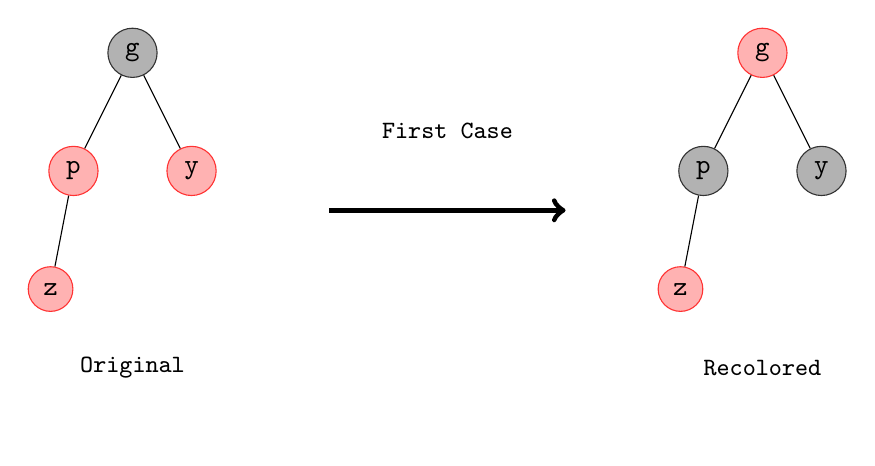
\begin{tikzpicture}[
          level distance=15mm, sibling distance=15mm,
          every node/.style={circle, draw, minimum size=8mm, font=\ttfamily\small}
        ]
        
        \begin{scope}[xshift=-4cm, every node/.style={circle, draw=blue!80, fill=blue!20, font =\ttfamily}]
            \node[circle, draw=black!80, fill=black!30] {g}
                child {node [circle, draw=red!80, fill=red!30]{p}
                    child[left] {
                        node [circle, draw=red!80, fill=red!30]{z}
                    } 
                }
                child{node[circle, draw=red!80, fill=red!30]{y}}
            ;
        \end{scope}
        
        \begin{scope}[xshift=4cm, every node/.style={circle, draw=blue!80, fill=blue!20, font=\ttfamily}]
            \node[circle, draw=red!80, fill=red!30] {g}
                child {node [circle, draw=black!80, fill=black!30]{p}
                    child[left] {
                        node [circle, draw=red!80, fill=red!30]{z}
                    } 
                }
                child{node[circle, draw=black!80, fill=black!30]{y}}
            ;
        \end{scope}
        
        \draw[->, very thick, line width=2pt] (-1.5,-2.0) -- (1.5,-2.0) 
            node[midway, above, yshift=0.2pt, draw=none, fill=none] {First Case};
        
                \node[draw=none, fill=none] at (-4, -4) {\textbf{Original} };
        \node[draw=none, fill=none] at (4, -4) {\textbf{Recolored} };
        
        \end{tikzpicture}
        \end{center} 
        \item \textit{\textbf{Second Case:} The uncle is black and the inserted node is a right child.}

        In this scenario, node $z$ is inserted as red, its parent $p$ is also red, while the uncle is black. Furthermore, $z$ is a right child of $p$, and $p$ is a left child of the grandparent, $g$.

        Since the uncle is black, we cannot resolve the issue with a simple recoloring. To handle the imbalance created by $z$'s position as a right child, we apply a \textbf{left rotation} on its parent, $p$. This rotation transforms the current problem into the configuration of the \textbf{Third Case}, which is simpler to resolve.

        This rotation repositions the nodes, effectively preparing the structure for the final adjustments described in the next step.
        \begin{center}
        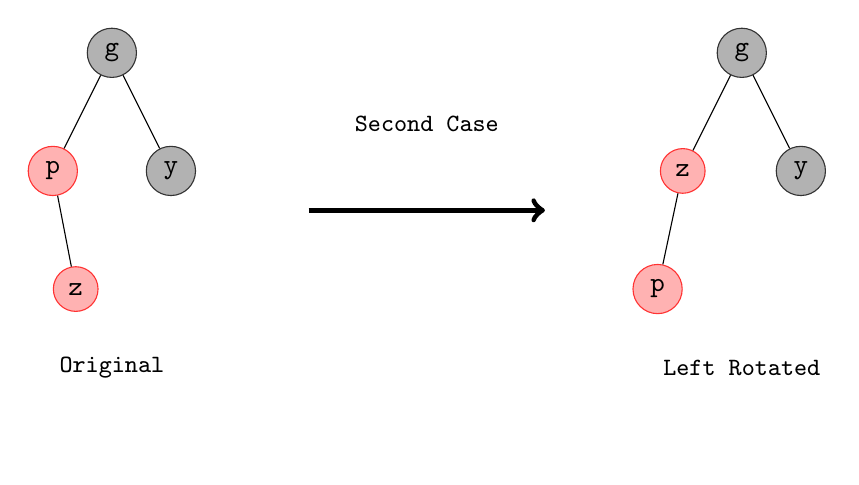
\begin{tikzpicture}[
          level distance=15mm, sibling distance=15mm,
          every node/.style={circle, draw, minimum size=8mm, font=\ttfamily\small}
        ]
        
        \begin{scope}[xshift=-4cm, every node/.style={circle, draw=blue!80, fill=blue!20, font =\ttfamily}]
            \node[circle, draw=black!80, fill=black!30] {g}
                child {node [circle, draw=red!80, fill=red!30]{p}
                    child[right] {
                        node [circle, draw=red!80, fill=red!30]{z}
                    } 
                }
                child{node[circle, draw=black!80, fill=black!30]{y}}
            ;
        \end{scope}
        
        \begin{scope}[xshift=4cm, every node/.style={circle, draw=blue!80, fill=blue!20, font=\ttfamily}]
            \node[circle, draw=black!80, fill=black!30] {g}
                child {node [circle, draw=red!80, fill=red!30]{z}
                    child[left] {
                        node [circle, draw=red!80, fill=red!30]{p}
                    } 
                }
                child{node[circle, draw=black!80, fill=black!30]{y}}
            ;
        \end{scope}
        
        \draw[->, very thick, line width=2pt] (-1.5,-2.0) -- (1.5,-2.0) 
            node[midway, above, yshift=0.2pt, draw=none, fill=none] {Second Case};
        
        \node[draw=none, fill=none] at (-4, -4) {\textbf{Original} };
        \node[draw=none, fill=none] at (4, -4) {\textbf{Left Rotated} };
        
        \end{tikzpicture}
        \end{center}
\item \textit{\textbf{Third Case:} The uncle is Black and $z$ is a left child.}

Since the uncle is black, it is considered stable. Therefore, the imbalance caused by $z$ can be resolved by applying a \textbf{right rotation} on the grandparent, $g$, and performing a \textbf{recoloring}.
        \begin{center}
        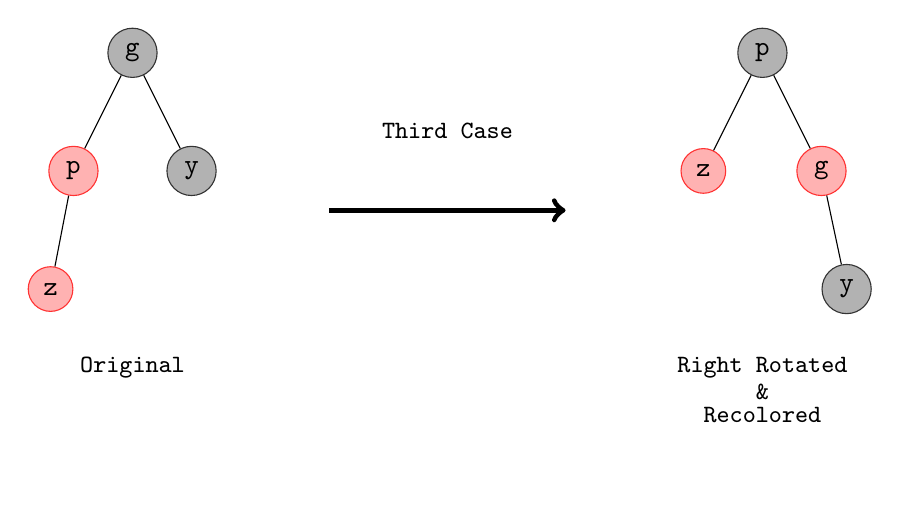
\begin{tikzpicture}[
          level distance=15mm, sibling distance=15mm,
          every node/.style={circle, draw, minimum size=8mm, font=\ttfamily\small}
        ]
        
        \begin{scope}[xshift=-4cm, every node/.style={circle, draw=blue!80, fill=blue!20, font =\ttfamily}]
            \node[circle, draw=black!80, fill=black!30] {g}
                child {node [circle, draw=red!80, fill=red!30]{p}
                    child[left] {
                        node [circle, draw=red!80, fill=red!30]{z}
                    } 
                }
                child{node[circle, draw=black!80, fill=black!30]{y}}
            ;
        \end{scope}
        
        \begin{scope}[xshift=+4cm, every node/.style={circle, draw=blue!80, fill=blue!20, font=\ttfamily}]
            \node[circle, draw=black!80, fill=black!30] {p}
                child {node [circle, draw=red!80, fill=red!30] {z}}
                child {node [circle, draw=red!80, fill=red!30] {g}
                    child[right] {
                        node [circle, draw=black!80, fill=black!30]{y}
                    } 
                };
        \end{scope}
        
        \draw[->, very thick, line width=2pt] (-1.5,-2.0) -- (1.5,-2.0) 
            node[midway, above, yshift=0.2pt, draw=none, fill=none] {Third Case};
                
        \node[draw=none, fill=none] at (-4, -4) {\textbf{Original} };
        \node[draw=none, fill=none] at (4, -4) {\textbf{Right Rotated}};
        \node[draw=none, fill=none] at (4, -4.3) {\textbf{\&}};
        \node[draw=none, fill=none] at (4, -4.6) {\textbf{Recolored}};
        
        \end{tikzpicture}
        \end{center}

        \end{itemize}
        \item \underline{\textbf{Function Insert:}} 
        
        Similar to the other implementations, the \texttt{Insert} function for the RBT handles two cases: if the word already exists in the tree, it simply adds the document ID to the list. Otherwise, it adds a new node as a leaf. For the RBT, at the end of this process, the tree is rebalanced using the \texttt{FixInsert} function.
    \end{itemize}        





    


\subsection{General Functions}
Since BST, AVL, and Red-Black trees are all binary trees, they naturally share similar functions due to their fundamentally similar structure. Therefore, the \texttt{create}, \texttt{search}, and \texttt{destroy} functions are the same for all of them.

\begin{itemize}
    \item \underline{\textbf{Create Function:}}
    
    The \texttt{create} function is responsible for creating the tree by initializing the root and the NIL node (used in the Red-Black Tree) as null pointers, thereby preventing invalid memory access.\newline
    
    \item \underline{\textbf{Search Function:}}
    
    By definition, a binary tree is constructed so that for any given node, smaller values are stored in the left subtree and larger values in the right. Based on this principle, the search operation is executed efficiently by leveraging the structure's inherent order.
    
    The search algorithm traverses the tree by comparing the target word with the keys in each node, using a \texttt{compare} function that returns the difference of the first diverging letter based on the ASCII table. Depending on this return value, the algorithm decides whether to traverse to the left or right child. This process repeats until the word is found or a null pointer is reached (a child of a leaf), indicating the word is not in the tree. If the word is located, the function returns a structure containing the result information. For statistical purposes, a timer is used to measure the search execution time.
    
    Regarding complexity, the algorithm's efficiency is closely tied to the tree's height, with a complexity of \(O(h)\), where \(h\) is the height of the binary tree. In the best-case analysis, when the tree is perfectly balanced, the complexity is \(O(\log n)\), where \(n\) is the number of nodes. On the other hand, in the worst case—when the tree degenerates into the shape of a linked list—the search has a complexity of \(O(n)\), this applies to the BST, which does not self-balance.\newline

    \item \underline{\textbf{Destroy Function:}}

    Finally, the \texttt{destroy} function is responsible for freeing all memory allocated by the binary tree structure. To accomplish this, it uses a helper function called \texttt{deleteTreeRecursive}, which employs a Post-Order Depth-First Search (DFS). Through recursion, it deletes nodes from the leaves up to the root. Once the node deallocation process is complete, the tree's root pointer is reset to null, ensuring the structure is completely cleared.

\end{itemize}




